% Supplementary Material for PAPER4_PIEZO_DRAFT.tex
%   S.1  cubic consistency condition and open-circuit rank-1 coefficient
%   S.2  inverse G2 cross-checks
%   S.3  F-F FE discriminator and mixed-BC outer-only ground
%   S.4  wide-axis admittance figure
%   S.5  thickness-ratio sweep and Y at 1/8, 1/5
%   S.6  cluster job provenance
%   S.7  mixed-edge C-F / F-C closed form
%   S.8  frequency-precision sweep and lab noise floor
%   S.9  three-dimensional n >= 1 finite-element check
%   S.10 Liu 2002 solid-disk CPT (Tables 2 and 6)
\documentclass[11pt]{article}
\usepackage[T1]{fontenc}
\usepackage{lmodern}
\usepackage[margin=1in,letterpaper]{geometry}
\usepackage{amsmath,amssymb,booktabs,array,xcolor}
\usepackage{textcomp}
\usepackage[hidelinks]{hyperref}
\usepackage{graphicx}
\graphicspath{{paper_figures/}{./}{../paper_figures/}}
\usepackage{caption}
\captionsetup{font=small,labelfont=bf,skip=4pt}
\usepackage{placeins}
\usepackage{seqsplit}
\renewcommand{\topfraction}{0.9}
\renewcommand{\bottomfraction}{0.85}
\renewcommand{\textfraction}{0.07}
\renewcommand{\floatpagefraction}{0.85}
\setcounter{topnumber}{4}
\setcounter{bottomnumber}{4}
\setcounter{totalnumber}{8}
\emergencystretch=2.5em
\raggedbottom

\renewcommand{\thesection}{S.\arabic{section}}
\renewcommand{\thesubsection}{S.\arabic{section}.\arabic{subsection}}
\renewcommand{\thetable}{S.\arabic{table}}
\renewcommand{\thefigure}{S.\arabic{figure}}
\renewcommand{\theequation}{S.\arabic{equation}}

\newcommand{\eebar}{\bar{e}_{31}}
\newcommand{\Xibar}{\bar{\Xi}_{33}}
\newcommand{\fn}[1]{\texttt{\seqsplit{#1}}}

\title{\bfseries Supplementary Material:\\
Exact Radial-Determinant Frequencies of a Piezoelectric Annular Plate,
and Inverse Recovery of $e_{31}$ from Open-Circuit Flexure}
\author{Garrek McCune$^{a,*}$, Daniel Stutts$^{a}$\\
\small\itshape $^a$Mechanical and Aerospace Engineering,\\
Missouri University of Science and Technology, Rolla, MO 65409, USA\\
\small\upshape $^*$Corresponding author. E-mail: ghmkfh@umsystem.edu}
\date{DRAFT --- \today}

\begin{document}
\maketitle
\noindent Main text contains no job numbers; they are listed in
\S\ref{sec:jobs}.

\section{Cubic consistency condition}
\label{sec:s1}
Each layer carries $\varphi=\pm\bar\varphi f(s)$, $s=\lvert z\rvert-h\in[0,h_1]$,
with $f(0)=f(h_1)=0$ (mirrored so that the two layers' moments add). The
thickness-integrated electric enthalpy of one layer is
$-\eebar I_1\bar\varphi\nabla^2w-\tfrac12\Xibar I_2\bar\varphi^2
-\tfrac12\Xi_{11}I_3\lvert\nabla\bar\varphi\rvert^2$ plus the elastic
part, with $I_1=\int zf'\,\mathrm dz=-\int f\,\mathrm ds$,
$I_2=\int f'^2\,\mathrm ds$, $I_3=\int f^2\,\mathrm ds$. Stationarity in
$w$ and $\bar\varphi$ gives the flexural equation with piezo moment
coefficient $K=-2\eebar I_1$ (two layers) and the electrical equation
$\Xi_{11}I_3\Delta\bar\varphi-\Xibar I_2\bar\varphi-\eebar I_1\Delta
w=0$; the insulated edge $\partial\bar\varphi/\partial r=0$ is its
natural condition. The long-wave increment per layer is
$(\eebar I_1)^2/(\Xibar I_2)\le h_1^3\eebar^{\,2}/(12\Xibar)$ by
Cauchy--Schwarz, with equality only for $f'$ linear in $s$, i.e.\ the
quadratic bubble $f=4s(h_1-s)/h_1^2$ of the main text: $I_1=-2h_1/3$,
$I_2=16/(3h_1)$, $I_3=8h_1/15$, so $K=\tfrac43h_1\eebar$ and the
normalized electrical equation is
$a\Delta\bar\varphi-\bar\varphi+c\Delta w=0$ with
$a=h_1^2\Xi_{11}/(10\Xibar)$, $c=h_1^2\eebar/(8\Xibar)$. The sine of
Duan, Quek and Wang \cite{duan2005} gives $K=(4/\pi)h_1\eebar$; under
this projection its long-wave increment is $96/\pi^4$ of exact, and under
their thickness-integrated Gauss-law closure ($a=h_1^2\Xi_{11}/(\pi^2\Xibar)$,
$c=h_1^2\eebar/(2\pi\Xibar)$) it is $12/\pi^2$ of exact. The earlier
version of this paper used that closure; the solver keeps it as a
switch (\texttt{projection='duan'}), and it reproduces every earlier
number bit-for-bit. Positing $\bar\varphi=\chi\bar w$ with $\chi$
independent of $r$ gives $\lambda=\chi/(a\chi+c)$ from the electrical
equation and $(d_1+d_2)\lambda^2+K\chi\lambda-A_2\omega^2=0$ from the
flexural one; eliminating $\lambda$ gives the cubic
$Ka\chi^3+(d_1+d_2+Kc-A_2\omega^2a^2)\chi^2-2A_2\omega^2ac\,\chi
-A_2\omega^2c^2=0$ (Duan, Quek and Wang's Eq.~17a is the same cubic up
to a constant factor, with their coefficients). Each of the three roots $(\chi_i,\lambda_i)$ depends on
the trial frequency $\omega$. For each root the radial problem is
$\Delta\bar w-\lambda_i\bar w=0$, with Bessel pair $(J_n,Y_n)$ or
modified pair $(I_n,K_n)$ according to the sign of $\lambda_i$. The
general short-circuit solution is the sum over all three branches. The
limit $\eebar\to0$ is singular (leading and two subleading coefficients
of the cubic vanish together), so the elastic bilayer is a separate
$4\times4$.

The open-circuit rank-1 coefficient of the main text,
\begin{equation}
\alpha=\frac{4\eebar^2 (h+h_1/2)^2h_1}{\Xibar(r_o^2-r_i^2)},
\end{equation}
is the unique sign that raises the first free--free $n=0$ root. It is
the product of the moment arm of $M_p$ and the charge arm of $Q$, both
$h+h_1/2$ (the bus charge is $-\partial\mathcal H/\partial V$ of the same
enthalpy); the earlier outer-face charge arm $h+h_1$ made $\alpha$ too
large by $(h+h_1)/(h+h_1/2)$. On a
mixed edge the same $\alpha S$ is added only where $M_{rr}=0$ is
imposed (the free edge). Driven
$Q/V$ uses the same $4\times4$ with right-hand side
$M_p=2\eebar(h+h_1/2)V$ on both moment rows. An independent bisection
of this $Q/V$ recovers the open-circuit root to $9\times10^{-15}$
relative.

\section{Inverse on-branch cross-check}
\label{sec:s2}
For the two clamped--clamped short-circuit recoveries, the product
$(\mathrm{d}\omega/\mathrm{d}p)(\mathrm{d}p/\mathrm{d}\omega)$ on the
solution branch is $0.999999$ ($e_{31}$) and $1.000008$ ($E$).
Propagated uncertainties at $0.10\%$ frequency precision are ten times
the $0.01\%$ values in main-text Table~4: $0.246\%$ of $E$, $3303\%$ of
short-circuit $e_{31}$, and $8.70\%$ of open-circuit $e_{31}$ at
$h_1/2h=1/12$.

The sequential recovery (main text \S6) was run at full production
precision (\texttt{dps=100}). Round trip:
$\hat E=2.000000009\times10^{11}\,\mathrm{Pa}$
($4.5\times10^{-9}$ relative), then, holding $\hat E$,
$\hat e_{31}=-4.099999346\,\mathrm{C\,m^{-2}}$
($1.6\times10^{-7}$ relative); both below the $10^{-6}$ bar. On-branch
sensitivities at $h_1/2h=1/12$:
$\mathrm{d}\omega_{\mathrm{SC}}/\mathrm{d}E=5.678\times10^{-9}\,\mathrm{rad\,s^{-1}\,Pa^{-1}}$,
$\mathrm{d}\omega_{\mathrm{OC}}/\mathrm{d}e_{31}=-2.1375\,\mathrm{rad\,s^{-1}\,m^2\,C^{-1}}$,
$\mathrm{d}\omega_{\mathrm{OC}}/\mathrm{d}E=1.494\times10^{-9}\,\mathrm{rad\,s^{-1}\,Pa^{-1}}$,
giving an implicit $\mathrm{d}e_{31}/\mathrm{d}E|_{\omega_{\mathrm{OC}}}=6.992\times10^{-10}\,\mathrm{C\,m^{-2}\,Pa^{-1}}$.
At $0.01\%$ frequency precision this splits the $1.21\%$ total of
main-text Table~4 into a $0.870\%$ direct term and a $0.839\%$ term from
propagating $\hat E$'s own $0.0246\%$ uncertainty, added in quadrature;
at $0.10\%$ frequency precision the same split gives $8.70\%$ and
$8.39\%$, total $12.08\%$. The recovered $\hat e_{31}$ is on the printed
branch, not the reflection twin at $22.0\,\mathrm{C\,m^{-2}}$. The
negative control substitutes the clamped--clamped
open-circuit root for the free--free one in the second step:
$\hat e_{31}=-4.09975379\,\mathrm{C\,m^{-2}}$ still solves (sign flip
present), but
$\mathrm{d}\omega_{\mathrm{SC}}/\mathrm{d}e_{31}|_{\hat E}=-2.062\times10^{-2}\,\mathrm{rad\,s^{-1}\,m^2\,C^{-1}}$
propagates to $330.3\%$ of $e_{31}$ at $0.01\%$ frequency precision --
the single-parameter clamped--clamped figure of
main-text Table~4, confirming the control fails as required.

\section{Finite-element discriminator and mixed electrical boundary}
\label{sec:s3}
Axisymmetric PLANE223, KEYOPT(1)=1001, millimetre--newton--second--tonne,
relative permittivity, one mesh for every electrical condition compared.
Mode~1 is the numerical rigid body ($\le 0.004\,\mathrm{Hz}$). Mode~2 is
bending: transverse displacement same sign and magnitude at the host top
and bottom at $r=r_o$; radial displacement opposite. The ratio of those
components at $h_1/2h=1/12$ is $19.71$ (both-faces short-circuit) and
$20.06$ (open-circuit). Open-circuit mechanical amplitudes are
smaller under unity-normalization because VOLT participates in the norm;
the ratio is the identifier. Every number in this section is from the
$e_{31}=-4.1\,\mathrm{C\,m^{-2}}$ rerun of the decks (job 2532086,
\S\ref{sec:jobs}); coupling-off decks carry no $e_{ij}$ and were not
rerun.

The outer-only-ground deck (VOLT$=0$ on $z=\pm(h+h_1)$, interface free)
gives $121.859\,\mathrm{Hz}$. That is $2.56\%$ above true both-faces
short-circuit ($118.816\,\mathrm{Hz}$), and $0.60\%$ above open-circuit,
and is not used as the short-circuit baseline in the main text.
Coupling-off is $118.810\,\mathrm{Hz}$.

At $h_1/2h=1/8$: mode~2 is $124.722\,\mathrm{Hz}$ open-circuit,
$121.364\,\mathrm{Hz}$ short-circuit, discriminator ratio $20.20$ and
$19.70$. At $1/5$: mode~2 is $132.183\,\mathrm{Hz}$ open-circuit,
$127.105\,\mathrm{Hz}$ short-circuit, discriminator ratio $20.43$ and
$19.70$. All runs show mode~1 at $0\,\mathrm{Hz}$ (rigid body), end
with \texttt{RUN COMPLETED}, and report zero in the MAPDL
\texttt{NUMBER OF ERROR MESSAGES ENCOUNTERED} line. (The original
$+4.1$ decks carried the literal string \texttt{*** ERROR ***} in a
pre-registration comment, which a queue script's text scan once
misreported as a failure; the rerun decks neutralize that token.)

The same pair with the piezo through-thickness division count doubled
from 2 to 4, leaving radial divisions, host through-thickness divisions,
units, and electrical BC unchanged, moves the three splits by at most
$4\times10^{-5}$ of their value ($1.9438\%$, $2.7661\%$, $3.9951\%$
against $1.9438\%$, $2.7662\%$, $3.9953\%$). The finite-element splits
are $99.7\%$, $99.6\%$ and $99.5\%$ of the tabulated closed-form
$\Delta_{\mathrm{OC}}$, and $99.7\%$, $99.7\%$ and $99.7\%$ of the
interior-enriched open-circuit root over the short-circuit $6\times6$
($1.9493\%$, $2.7747\%$, $4.0080\%$), which is the like-for-like
quantity.

\paragraph{Sign control.} The same decks were first run with
$e_{31}=+4.1\,\mathrm{C\,m^{-2}}$ ($\eebar=-4.85$; jobs 2491761,
2491831, 2494226, 2494665, 2495593 of \S\ref{sec:jobs}). Their splits,
$0.2795\%$, $0.4047\%$ and $0.6002\%$ (F--F) and $0.2593\%$ (C--F),
are $99.9\%$, $99.9\%$, $99.9\%$ and $98.9\%$ of the closed form at that
sign. Across the two signs the finite-element F--F split grows by
factors of $6.95$, $6.84$ and $6.66$ at the three ratios, against
closed-form factors of $6.97$, $6.85$ and $6.68$; the open-circuit
update tracks $\eebar^{\,2}$, not one calibrated point. An earlier
version of this model took the bus charge at the outer face (arm
$h+h_1$); against it the $+4.1$ finite elements recovered
$93\%/90\%/86\%$, which is the charge-arm ratio
$(h+h_1/2)/(h+h_1)=0.929/0.900/0.857$ and not a mesh effect.

\section{Wide-axis admittance}
\label{sec:s4}
\begin{figure}[ht]
\centering
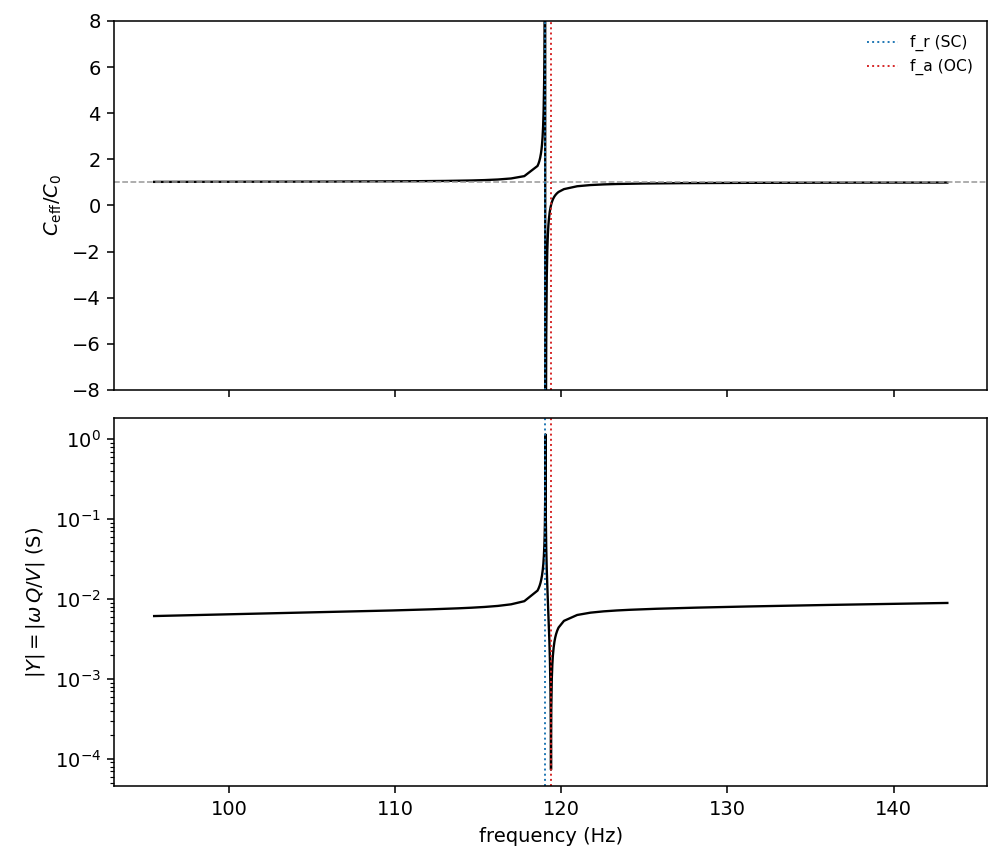
\includegraphics[width=0.92\linewidth]{piezo_p4_admittance_sweep.png}
\caption{Driven $C_{\mathrm{eff}}/C_0$ and $|Y|$ on $95$--$145\,\mathrm{Hz}$
at $h_1/2h=1/12$. The pole and zero of the first $n=0$ pair differ by
$1.95\%$; main-text Fig.~4 zooms $116$--$122.5\,\mathrm{Hz}$.}
\label{fig:s1}
\end{figure}

A harmonic PLANE223 run on the same mesh (job 2532146; $1\,\mathrm{V}$
on the outer-bus master, KEYOPT(1)=1001 charge reaction,
$118.55$--$122\,\mathrm{Hz}$ in $70$ substeps) places the
$|Y|$ peak at $118.80\,\mathrm{Hz}$, the charge changing sign through the
pole between $118.80$ and $118.85\,\mathrm{Hz}$ ($118.82\,\mathrm{Hz}$ by
linear interpolation of $1/Q$), and the charge-zero at
$121.126\,\mathrm{Hz}$, against the modal pair $118.816$ /
$121.126\,\mathrm{Hz}$. The same deck in job 2532086 swept only the
narrower window of the $e_{31}=+4.1$ run and did not reach the zero; it
is superseded. At $+4.1$ (job 2494863) the same construction placed the
pair at $118.79$ / $119.13\,\mathrm{Hz}$ against $118.811$ /
$119.143\,\mathrm{Hz}$. An earlier harmonic dump (job 2494669) used
the current label \texttt{AMPS}, which is KEYOPT(1)=101, and returned
a numerical-zero bus current at every frequency; that run is not a
disproof of the pole/zero.
\FloatBarrier

\section{Thickness-ratio sweep and other-ratio admittance}
\label{sec:s5}
Figure~\ref{fig:s2} is the closed-form $h_1/2h$ sweep that sits
underneath main-text Table~2 and Fig.~2: eleven ratios from $1/40$ to
$1/4$, linear-potential open-circuit $4\times4$ against the elastic
bilayer. The three Duan Table~4 ratios (red) lie on the curve. The
thin-layer intercept $\Delta_{\mathrm{OC}}/(h_1/2h)\to 0.25$ is the
leading $h_1$ scaling of the rank-1 coefficient $\alpha$ (the same limit
under either charge arm, since $h_1\to0$). The bottom
panel is the single-parameter $e_{31}$ G2 at $0.01\%$ frequency
precision (host $E$ known exactly); it is $2.60\%$ at $1/40$ and
$0.40\%$ at $1/4$.

\begin{figure}[ht]
\centering
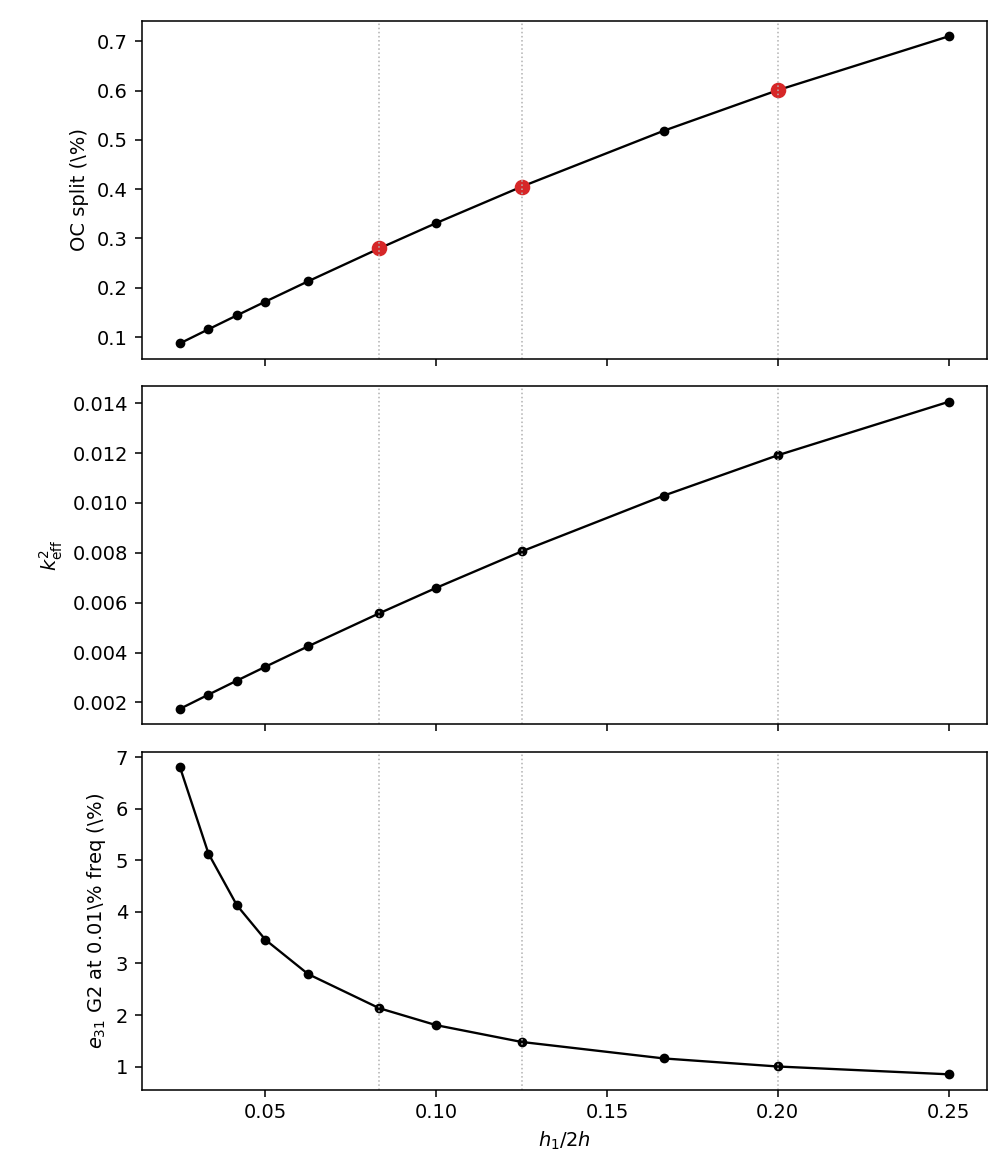
\includegraphics[width=0.92\linewidth]{piezo_p4_h1_ratio_sweep.png}
\caption{Closed-form F--F $n=0$ open-circuit split, $k_{\mathrm{eff}}^2$,
and $e_{31}$ G2 versus $h_1/2h$. Red markers are the three Duan Table~4
ratios already in the main text.}
\label{fig:s2}
\end{figure}

Figure~\ref{fig:s3} is the driven $Q/V$ problem at the other two
Table~4 ratios. Independent bisection of $Q/V$ recovers
\texttt{oc\_ff\_bisect} to $1.7\times10^{-14}$ ($1/8$) and
$3\times10^{-16}$ ($1/5$); $k_{\mathrm{eff}}^2$ from the driven
pole/zero is $0.0533$ and $0.0757$. $C_0=6.66\,\mathrm{\mu F}$ at
$1/8$ and $4.16\,\mathrm{\mu F}$ at $1/5$. Off-resonance
Butterworth--van Dyke shape: $C_{\mathrm{eff}}/C_0=1.135$ at
$0.55\,\omega_{\mathrm{el}}$ and $0.797$ at $1.08\,\omega_{\mathrm{OC}}$
at $1/8$; $1.201$ and $0.740$ at $1/5$.

\begin{figure}[ht]
\centering
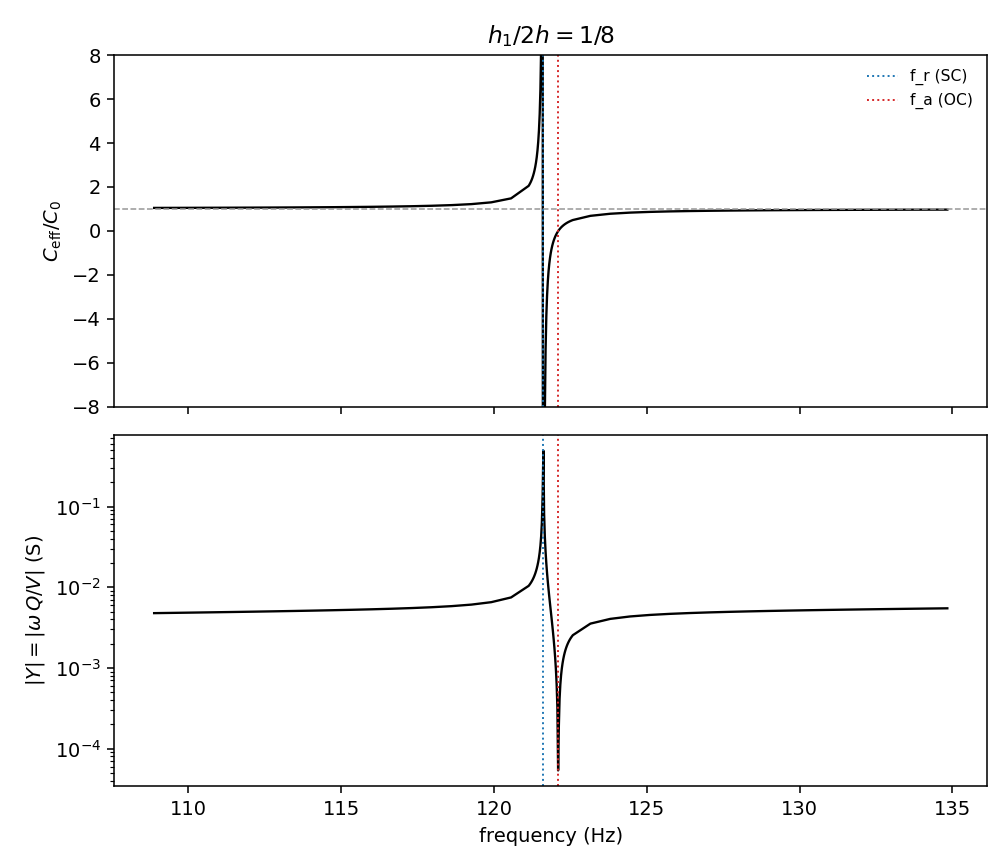
\includegraphics[width=0.48\linewidth]{piezo_p4_ff_admittance_sweep_h18.png}
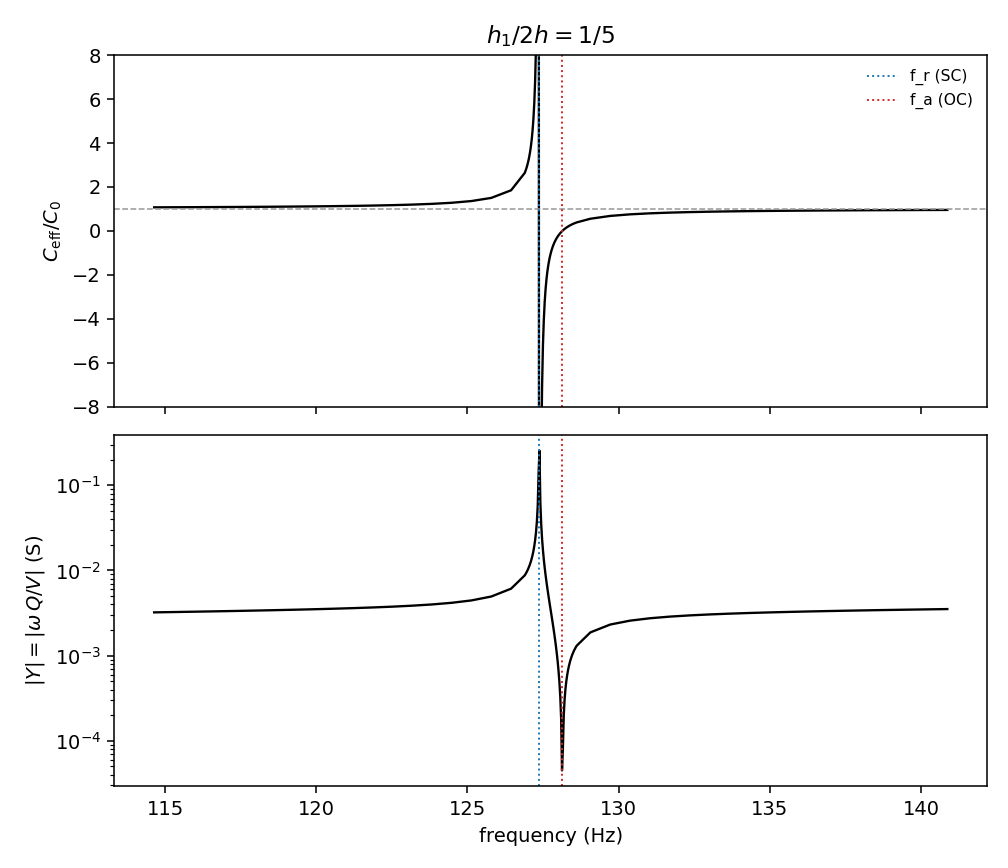
\includegraphics[width=0.48\linewidth]{piezo_p4_ff_admittance_sweep_h15.png}
\caption{Driven $C_{\mathrm{eff}}/C_0$ and $|Y|$ at $h_1/2h=1/8$ (left)
and $1/5$ (right). Pole at the elastic/short-circuit root, zero at the
open-circuit root, same linear-potential operator as main-text Fig.~4.}
\label{fig:s3}
\end{figure}
\FloatBarrier

\section{Cluster job provenance}
\label{sec:jobs}
All jobs on The Mill \cite{mill2024}, solver snapshot
\texttt{2026-07-10.s10}. Piezoelectric paths are new and unused by the
elastic default. Jobs up to 2531012 used $e_{31}=+4.1\,\mathrm{C\,m^{-2}}$;
the paper's numbers are from the $e_{31}=-4.1$ rerun described at the
end of this section, and the earlier jobs are kept as the sign control
of \S\ref{sec:s3}.

\begin{itemize}
\item 2489140 --- clamped--clamped Table~4 gate, 27/27, worst $-0.0476\%$.
\item 2490706 --- F--F coupling-off and outer-only-ground decks at
      $h_1/2h=1/12$.
\item 2490848 --- F--F outer-only-ground at $h_1/2h=1/8$ and $1/5$.
\item 2491531 --- clamped--clamped short-circuit inverse of $E$ and $e_{31}$.
\item 2491661 --- F--F open-circuit python archival, deploy miss
      (package lacked the open-circuit method); superseded by 2491764.
\item 2491761 --- F--F open-circuit finite elements, mode~2 $=119.143\,\mathrm{Hz}$.
\item 2491764 --- F--F open-circuit inverse archival, all gates passed.
\item 2491831 --- both-faces short-circuit finite elements, mode~2 $=118.811\,\mathrm{Hz}$.
\item 2491920 --- driven $Y(\omega)$ archival, all gates passed,
      $k_{\mathrm{eff}}^2=0.005997133$.
\item 2494216 --- sequential $E$-then-$e_{31}$ inverse archival at full
      \texttt{dps=100}, $h_1/2h=1/12$; SENTINEL PASS\_ALL, bit-identical
      to the in-sandbox validation run.
\item 2494226 --- F--F open-circuit and both-faces short-circuit finite
      elements at $h_1/2h=1/8$ and $1/5$, cloned from 2491761/2491831.
\item 2494665 --- lever 8 mesh refinement, NDIV\_ZP $2\to 4$ on the
      fair OC/scboth pair at all three Table~4 ratios; splits
      unchanged.
\item 2494667 --- lever 2 $h_1/2h$ sweep archival, SENTINEL PASS\_ALL,
      bit-identical to the in-sandbox run.
\item 2494668 --- lever 5 driven $Y(\omega)$ at $1/8$ and $1/5$
      archival, SENTINEL PASS\_ALL, bit-identical to the in-sandbox run.
\item 2494669 --- lever 9 first harmonic dump; MAPDL clean but
      \texttt{RF,AMPS} identically zero. Superseded by 2494863.
\item 2494863 --- lever 9 v2 harmonic $Y$ at $1/12$, \texttt{RF,CHRG};
      pole $118.79\,\mathrm{Hz}$, zero $119.13\,\mathrm{Hz}$.
\item 2494864 --- lever 3 other-constant inverses, SENTINEL PASS\_ALL.
\item 2494865 --- lever 1 $n=0$ overtones; one overtone in
      $(800,4000)\,\mathrm{rad\,s^{-1}}$ ($+0.137\%$ split). Pre-registered
      bar of two overtones in that window not met.
\item 2494945 --- lever 1 wide scan $(800,15000)\,\mathrm{rad\,s^{-1}}$,
      SENTINEL PASS\_ALL; second overtone $8515.06$ vs
      $8516.48\,\mathrm{rad\,s^{-1}}$ ($+0.017\%$).
\item 2494866 --- lever 4 F--F $E$ channel, SENTINEL PASS\_ALL,
      $0.025\%$ of $E$ at $0.01\%$ freq on both elastic and OC.
\item 2495528 --- lever 10 C--F / F--C mixed-edge archival,
      SENTINEL PASS\_ALL, bit-identical to the in-sandbox
      \texttt{dps=60} run.
\item 2495593 --- optional C--F FE, clones of 2491761/2491831 with
      inner $U_X=U_Y=0$ only. scboth $67.071\,\mathrm{Hz}$, OC
      $67.245\,\mathrm{Hz}$, $+0.259\%$ ($98.9\%$ of the consistent
      closed-form $+0.262\%$; $92\%$ of the Gauss-law $+0.282\%$). Both \texttt{RUN COMPLETED}, 0 MAPDL errors.
\item 2530336 --- first submission of the three-dimensional $n\ge1$
      queue (\S\ref{sec:s9}); no deck ran (the cluster had retired the
      ANSYS 2024~R2 module that every earlier finite-element job used).
\item 2530423 --- three-dimensional $n\ge1$ queue, ten SOLID226 decks,
      ANSYS 2025~R1, all \texttt{RUN COMPLETED}, 0 MAPDL errors, 0
      warnings (\S\ref{sec:s9}).
\item 2530553 --- thin-limit first pass, five bare-steel SOLID186 decks
      ($t=20$, $10$, $5\,\mathrm{mm}$), ANSYS 2025~R1, all
      \texttt{RUN COMPLETED}, 0 errors, 0 warnings (\S\ref{sec:s9}).
\item 2530671 --- thin-limit second pass, first submission; the
      $96\times288\times8$ decks exceeded the $64\,\mathrm{GB}$ memory
      request (in-core Block Lanczos, $67.8\,\mathrm{GB}$) and were killed;
      the added $t=10\,\mathrm{mm}$ coarse deck completed.
\item 2530784 --- thin-limit second pass, $96\times288\times8$ at $t=20$,
      $10$, $5\,\mathrm{mm}$, $100\,\mathrm{GB}$; all \texttt{RUN
      COMPLETED}, 0 errors (\S\ref{sec:s9}).
\item 2530987 --- Liu solid-disk decks, first version
      (\S\ref{sec:liu-disk}); both \texttt{RUN COMPLETED}, 0 errors. A
      displacement constraint on the central mesh hole blocked the $n=1$
      centre rotation and raised those modes by 2--7\%; superseded by
      2531012 and not used.
\item 2531012 --- Liu solid-disk decks with the hole free, SOLID226,
      ANSYS 2025~R1; both \texttt{RUN COMPLETED}, 0 errors
      (\S\ref{sec:liu-disk}).
\item 2495751 --- lever 16 frequency-precision sweep, SENTINEL
      PASS\_ALL, bit-identical to the in-sandbox run (F--F/C--F
      $e_{31}$ uncertainty curve plus the Boeringa--McCune lab
      floor).
\end{itemize}
\noindent\textbf{Consistent-projection rerun (2026-09-23).} Every
analytic job above (all but the finite-element jobs) used the Gauss-law
closure of \S\ref{sec:s1} and the outer-face charge arm. Every
package-based probe was re-run against the corrected solver
(default \texttt{projection='consistent'}; \texttt{projection='duan'}
reproduces the jobs above bit-for-bit), with only the hard-coded
open-circuit regression anchors of four probes moved to the new values.
All passed.

\noindent\textbf{$e_{31}=-4.1$ rerun (2026-09-24).} The piezoelectric
material bundle now carries $e_{31}=-4.1\,\mathrm{C\,m^{-2}}$ as printed
in Liu, Wang and Quek's and Duan, Quek and Wang's Table~1. Every
package-based probe behind a number in the main text or this document
was copied with $e_{31}=-4.1$ and every $e_{31}$ bracket moved to
$[-10,-1]\,\mathrm{C\,m^{-2}}$ (which excludes the reflection twin at
$22.0$). Magnitude windows that were pre-registered for $e_{31}=+4.1$
were multiplied by $(13.05/4.85)^2=7.24$ before the run. Regression
anchors that encoded $+4.1$ values were re-anchored to the $-4.1$ value
of an independent probe, never to the probe's own output: the
thickness-ratio sweep to the open-circuit and driven-$Q/V$ probes, the
driven $Q/V$ probes to the thickness sweep's free-vibration roots, and
the precision sweep to the open-circuit and mixed-edge probes, and the
wide overtone scan to the narrow one. Eleven
of the twelve gated probes end \texttt{SENTINEL PASS\_ALL}. The
twelfth, the narrow $n=0$ overtone scan, fails its pre-registered bar of
two overtones below $4000\,\mathrm{rad\,s^{-1}}$ exactly as job 2494865
did at $+4.1$ (there is one), and the wide scan finds the second; four
short scripts supply Table~4 in both closures, the clamped--clamped
short-circuit $e_{31}$ sensitivity, the interior-enriched open-circuit
root, and the solid-disk roots of \S\ref{sec:liu-disk}. The runs were made at
the probes' production precision (\texttt{dps} $40$--$100$) on a
two-core cloud workstation, not on the cluster; every earlier cluster
archival run of these probes reproduced its off-cluster run
bit-for-bit. The package test suite passes (110 tests; four of them pin
the $-4.1$ default, the Table~4 fundamentals, the open-circuit split and
the monolithic short-circuit root, and the solid-disk anchors of
\S\ref{sec:liu-disk} were moved to their $-4.1$ values). Finite elements: job 2532086 (ANSYS
2025~R1) reran every coupled deck of \S\ref{sec:s3}, \S\ref{sec:scf},
\S\ref{sec:s9} and \S\ref{sec:liu-disk} at $e_{31}=-4.1$, all
\texttt{RUN COMPLETED} with zero MAPDL errors; job 2532146 reran the
harmonic admittance deck on a window that contains the new zero.
Decks, text outputs, manifests, scorers and queue logs are in
\texttt{ansys/NewAnsys/} of the public code tree.

\section{Mixed-edge C--F / F--C closed form}
\label{sec:scf}
Paper~3 names inner then outer: C--F is clamped inner, free outer
(\texttt{bc\_inner='C'}, \texttt{bc\_outer='F'} in
\texttt{ring\_disk.py}). Methods on
\texttt{PiezoOutOfPlaneSolver}: \texttt{elastic\_cf\_det} /
\texttt{elastic\_fc\_det}, \texttt{cf\_coupled\_det} /
\texttt{fc\_coupled\_det}, \texttt{oc\_cf\_det} /
\texttt{oc\_fc\_det}. The mixed-edge engine recovers the existing
free--free and clamped--clamped determinants bit-exactly when both
edges are set equal. Bare-host $n=0$ roots match Paper~3's live
Frobenius solver at relative $4.45\times10^{-10}$ (C--F,
$410.074181\,\mathrm{rad\,s^{-1}}$) and $2.28\times10^{-10}$ (F--C,
$873.221632\,\mathrm{rad\,s^{-1}}$). SENTINEL PASS\_ALL
(\texttt{probe\_piezo\_p4\_cf\_mixed\_edge\_2026-09-16.py},
\texttt{dps=60}; $e_{31}=-4.1$ copy
\fn{probe\_piezo\_p4\_cf\_mixed\_edge\_e31m\_2026-09-24.py}): C--F
open-circuit $+1.826\%$, $k_{\mathrm{eff}}^2=0.0355$, $e_{31}$ G2
$0.93\%$ at $0.01\%$ frequency; F--C open-circuit $+0.0388\%$,
$k_{\mathrm{eff}}^2=0.00078$. Short-circuit $6\times6$ over the mixed
bilayer is $+0.0061\%$ (C--F) and $+0.0039\%$ (F--C). Inverse round-trip
on C--F $e_{31}$ is $4.0\times10^{-9}$. C--F finite elements (job
2532086): scboth $67.076\,\mathrm{Hz}$, OC $68.290\,\mathrm{Hz}$, split
$+1.811\%$ ($99.2\%$ of $+1.826\%$), no $0\,\mathrm{Hz}$ rigid body,
bending discriminator $45.5$ and $47.0$, 0 MAPDL errors. The $+4.1$
control (job 2495593) gave $+0.259\%$ against $+0.262\%$.
\texttt{SOLVER\_VERSION} remains \texttt{2026-07-10.s10}.

\section{Frequency-precision sweep and lab noise floor}
\label{sec:noisefloor}
Table~\ref{tab:noisefloor} extends the two-column ($0.01\%$, $0.1\%$)
$e_{31}$ inverse of the main-text open-circuit section and \S\ref{sec:scf} to an eight-point
log-spaced grid of assumed relative frequency error, on both the
free--free and clamped--free $n=0$ open-circuit channels, using the
identical linear-propagation formula (unchanged, not retuned):
$\delta e_{31}/e_{31}=(\delta\omega/\omega)\,\omega_{\mathrm{target}}
/(|\mathrm{d}\omega/\mathrm{d}e_{31}|\,e_{31,\mathrm{true}})$. The
lab-floor row (marked) is sourced from Table~3 of
\cite{boeringa2026}: an HP4294A impedance analyzer and a scanning
laser Doppler vibrometer measured the same five axial resonances of a
free--free PZT-4 rod specimen (a physically distinct specimen from
this ring, same material system), disagreeing by $0.12\%$,
$0.10\%$, $0.09\%$, $0.11\%$, and $0.09\%$ -- mean $0.102\%$. The
companion draft (\texttt{BoeringaMcCune2026-2.pdf}) was checked and
rejected as a source: its impedance-versus-SLDV table is internally
inconsistent (disagreements up to $26\%$ on a single mode) and
carries explicit placeholder text, so no number was taken from it.

\begin{table}[ht]
\centering
\caption{Propagated relative uncertainty in $e_{31}$ versus assumed
relative frequency error, $h_1/2h=1/12$. G0 round-trip error is
$4.0\times10^{-9}$ (bar $10^{-6}$) at every row; G\_anchor reproduces
the $0.01\%$ entries of main-text Table~4, and the $0.10\%$-scaled
figures of \S\ref{sec:s2}, to within $1\%$ relative; the linearity
self-check (every row equal to the base row scaled by the ratio of
assumed frequency errors) is exact to $10^{-9}$.}
\label{tab:noisefloor}
\small
\begin{tabular}{@{}lrr@{}}
\toprule
assumed rel.\ freq.\ error & F--F OC unc.\ of $e_{31}$ & C--F OC unc.\ of $e_{31}$ \\
\midrule
$0.001\%$  & $0.087\%$ & $0.093\%$ \\
$0.003\%$  & $0.261\%$ & $0.278\%$ \\
$0.01\%$   & $0.870\%$ & $0.928\%$ \\
$0.03\%$   & $2.610\%$ & $2.785\%$ \\
$0.1\%$    & $8.701\%$ & $9.282\%$ \\
$0.102\%$ (Boeringa--McCune floor \cite{boeringa2026}) & $8.875\%$ & $9.468\%$ \\
$0.3\%$    & $26.104\%$ & $27.847\%$ \\
$1\%$      & $87.013\%$ & $92.824\%$ \\
\bottomrule
\end{tabular}
\end{table}

Delivered as
\fn{Paper4\_Piezo/probe\_piezo\_p4\_lever16\_freq\_noise\_floor\_2026-09-16.py}
(LF) with matching submit script (\texttt{dps=60}, mirroring the
free--free/clamped--free probes' own settings); its $e_{31}=-4.1$ copy
(\texttt{\ldots\_e31m\_2026-09-24.py}) produced the table above,
SENTINEL PASS\_ALL. The $+4.1$ version was archived on the cluster (job
2495751) bit-identical to its off-cluster run. \texttt{SOLVER\_VERSION}
remains \texttt{2026-07-10.s10}.

\section{Three-dimensional $n\ge1$ finite-element check}
\label{sec:s9}
SOLID226 (KEYOPT(1)=1001) for host and skins, three glued volumes, host
with zero piezoelectric constants and relative permittivity~1, skins
PZT-4 poled $+z$; millimetre--newton--second--tonne, relative
permittivity. Half ring $0\le\theta\le\pi$, $U_Y=0$ on $y=0$: the
$\cos n\theta$ family at every $n$, three rigid modes left. Electrical
cases as in \S\ref{sec:s3}: coupling-off ($e_{ij}=0$), both-faces
short-circuit, and open-circuit (interfaces grounded, one coupled VOLT
set on both outer faces). Meshes $24\times72\times(2+1+1)$ and
$40\times144\times(4+2+2)$ (radial, circumferential, host and each
skin). Circumferential order is read from a discrete cosine transform of
$U_Z$ at $13$ angles on five radii; every scored mode has purity
$1.0000$. Coarse-to-fine changes are at most $0.025\%$ in frequency and
$0.2\%$ in the short-circuit shift. ANSYS 2025~R1 (job 2530423 at
$e_{31}=+4.1$; coupled decks rerun at $-4.1$ in job 2532086); the
axisymmetric coupling-off deck ran under 2024~R2, and the $n=0$
coupling-off root agrees with it to $0.0003\%$.
Every quantity below is a ratio of raw MAPDL frequencies. Criteria were
fixed before the run.

\begin{table}[ht]
\centering
\caption{Three-dimensional finite elements (fine mesh) against the
closed form, first radial root. Shift: short-circuit over coupling-off
minus one (finite elements) and short-circuit $6\times6$ over elastic
$4\times4$ minus one (closed form). Offset: coupling-off over the
elastic bilayer minus one. Open-circuit minus short-circuit is below
$3\times10^{-10}$ relative at every $n\ge1$.}
\label{tab:s9}
\small
\begin{tabular}{@{}lrrrrr@{}}
\toprule
$h_1/2h$, $n$ & FE shift & closed-form shift & FE/closed $-1$ & FE coupling-off (Hz) & offset \\
\midrule
$1/12$, 0 & $5.230\times10^{-5}$ & $5.212\times10^{-5}$ & $+0.3\%$ & 118.8105 & $-0.198\%$ \\
$1/12$, 1 & $4.929\times10^{-5}$ & $4.920\times10^{-5}$ & $+0.2\%$ & 276.6199 & $-1.022\%$ \\
$1/12$, 2 & $1.045\times10^{-5}$ & $1.048\times10^{-5}$ & $-0.3\%$ & 72.3441 & $-0.533\%$ \\
$1/12$, 3 & $1.367\times10^{-5}$ & $1.396\times10^{-5}$ & $-2.1\%$ & 172.2871 & $-0.647\%$ \\
$1/12$, 4 & $1.706\times10^{-5}$ & $1.742\times10^{-5}$ & $-2.1\%$ & 301.9394 & $-0.935\%$ \\
$1/5$, 0 & $5.300\times10^{-4}$ & $5.285\times10^{-4}$ & $+0.3\%$ & 127.0378 & $-0.262\%$ \\
$1/5$, 1 & $4.984\times10^{-4}$ & $4.978\times10^{-4}$ & $+0.1\%$ & 295.4942 & $-1.192\%$ \\
$1/5$, 2 & $1.059\times10^{-4}$ & $1.065\times10^{-4}$ & $-0.5\%$ & 77.4742 & $-0.604\%$ \\
$1/5$, 3 & $1.382\times10^{-4}$ & $1.417\times10^{-4}$ & $-2.5\%$ & 184.4153 & $-0.753\%$ \\
$1/5$, 4 & $1.722\times10^{-4}$ & $1.768\times10^{-4}$ & $-2.6\%$ & 322.9683 & $-1.097\%$ \\
\bottomrule
\end{tabular}
\end{table}

Against the pre-registered criteria: the axisymmetric control, mesh
convergence, the open-circuit/short-circuit coincidence at $n\ge1$, and
the shift ($\pm10\%$, all ten within $\pm2.6\%$; within $\pm1.2\%$ in the
$+4.1$ run, where the shift is $7.24$ times smaller) pass. The elastic
offset criterion, $|\text{offset}|\le1\%$ at $n=1$--$4$, fails at three
of eight points ($1/12$ $n=1$; $1/5$ $n=1$ and $4$). It was set on the
assumption that the offset would grow from its $n=0$ value with
frequency alone; the $n\ge1$ points instead carry an extra $-0.2\%$ to
$-0.46\%$ beyond a plane-wave transverse-shear and rotary-inertia
estimate, which accounts for the $n=0$ offset. The retired $Q_r$
free-edge row is $10.5\%$ off the finite elements at $1/12$, $n=1$.

\paragraph{Thin-limit follow-up.} To separate thickness physics from an
$n$-dependent error in the thin-plate operator, the same half ring was
run as bare steel ($E=200\,\mathrm{GPa}$, $\nu=0.3$, no skins) at full
thickness $t=20$, $10$ and $5\,\mathrm{mm}$ (SOLID186, full
integration). Kirchhoff roots scale exactly with $t$, so any offset that
survives $t\to0$ is an operator error. Each thickness was run on three
uniformly refined meshes, $24\times72\times2$, $48\times144\times4$, and
$96\times288\times8$ (the last $2.93\times10^{6}$ equations), and each
root was Richardson-extrapolated with its observed order $p$.
Table~\ref{tab:s9thin} gives the mesh-extrapolated
$\delta_n(t)=f_{\mathrm{FE}}/f_{\mathrm{K}}-1$ and the intercept $c$ of
the quadratic $\delta=c+at+bt^2$ through the three thicknesses.

\begin{table}[ht]
\centering
\caption{Bare steel annulus, first radial root, Richardson-extrapolated
mesh limit. $c_\infty$: quadratic extrapolation to $t=0$; $c_x$: the same
from the finest mesh without Richardson; $at$, $bt^2$ at
$t=20\,\mathrm{mm}$; $p$: observed convergence order at
$t=5\,\mathrm{mm}$.}
\label{tab:s9thin}
\small
\begin{tabular}{@{}rrrrrrrrr@{}}
\toprule
$n$ & $t=20$ & $t=10$ & $t=5$ & $c_\infty$ & $c_x$ & $at$ & $bt^2$ & $p$ \\
\midrule
0 & $-0.158\%$ & $-0.040\%$ & $-0.010\%$ & $-0.000\%$ & $+0.000\%$ & $-0.000\%$ & $-0.158\%$ & 3.3 \\
1 & $-0.918\%$ & $-0.361\%$ & $-0.161\%$ & $-0.014\%$ & $+0.013\%$ & $-0.481\%$ & $-0.422\%$ & 1.5 \\
2 & $-0.490\%$ & $-0.223\%$ & $-0.111\%$ & $-0.013\%$ & $+0.009\%$ & $-0.363\%$ & $-0.114\%$ & 1.5 \\
3 & $-0.583\%$ & $-0.236\%$ & $-0.106\%$ & $-0.005\%$ & $+0.009\%$ & $-0.346\%$ & $-0.231\%$ & 1.9 \\
4 & $-0.836\%$ & $-0.320\%$ & $-0.137\%$ & $-0.004\%$ & $+0.012\%$ & $-0.434\%$ & $-0.398\%$ & 2.1 \\
\bottomrule
\end{tabular}
\end{table}

Criteria were fixed before each run. A first pass on the two coarser
meshes was formally unresolved: its coarse-to-fine change at
$t=5\,\mathrm{mm}$ exceeded the $0.05\%$ bar at three orders, so its
intercept (then $+0.004\%$ to $+0.055\%$) was not scored. The second
pass added the finest mesh and required monotone ratio-2 convergence
with $1\le p\le8$ at every thickness and order (met at all fifteen
points), took the intercept from the Richardson limits in that case, and
required $|c|\le0.03\%$ at $n=0$--$4$: all five pass, with
$|c_\infty|\le0.014\%$. A separate criterion, fine-to-finest change at most
$0.02\%$, fails at two points ($t=5$, $n=1$ and $4$: $0.023\%$ and $0.024\%$) and does
not enter the intercept by the pre-registered rule. Convergence is
monotone from above, so the finest-mesh intercept $c_x$ and the
Richardson intercept $c_\infty$ bracket the limit; both are within
$0.015\%$ of zero at every order. An operator error of the size of the
$n\ge1$ excess in the main text would have given $c$ of $-0.2\%$ to
$-0.46\%$. The $n=0$ offset is quadratic in $t$ to three figures (ratios
$3.99$ and $3.97$ per halving). At $n\ge1$ the fitted linear term is as
large as or larger than the quadratic one, the signature of a free-edge
boundary layer rather than interior shear alone. The finest $t=5$ deck
printed one Block Lanczos ill-conditioning warning (test residual
$3.3\times10^{-3}$ at the $-1\,\mathrm{Hz}$ shift); its roots continue
the monotone sequence of the two coarser meshes, and no other deck
printed a warning or an error.


\section{Liu 2002 solid-disk short-circuit CPT}
\label{sec:liu-disk}

Liu, Wang and Quek \cite{liu2002} tabulated free-vibration frequencies of
a steel circular plate (no hole) with identical thickness-polarized PZT-4
skins on both faces, both faces of each skin short-circuited. Only their
classical-plate column $x_{\mathrm{kir}}$ is scored here; their Mindlin
and three-dimensional finite-element columns are not. Geometry of their
Tables~2 and~6: $r_0=0.6\,\mathrm{m}$, host half-thickness
$h=0.01\,\mathrm{m}$, skin thickness $h_1=0.002\,\mathrm{m}$
($r_0/h=60$); materials as their Table~1, including
$e_{31}=-4.1\,\mathrm{C\,m^{-2}}$, as in the main text.

The solid disk has its own determinant. Keeping only the centre-regular
Bessel function of each of the three $\chi$-branches of
Section~\ref{sec:s1} gives a $3\times3$; its rows are $w=w'=0$ (outer
edge clamped, Liu's Tables~2--5) or $w=M_r=0$ (simply supported, Tables
6--9), each with the short-circuit row $\phi'=0$. The annular $6\times6$
evaluated at $r_i=0$ is not this determinant, because its $Y_n$ and $K_n$
columns are singular there, and the annular solver refuses $r_i\le0$.
With $h_1=0$ the disk reduces to the $2\times2$ on $\{J_n,I_n\}$ of
McCune and Stutts \cite{mccune2026ring}, and it reproduces their
$\lambda^2$ for $n=0,1,2$, $m=1,2$, under both edge conditions, to
$5\times10^{-6}$. Roots were located by sampling the determinant on a
uniform grid ($800$ points from $50\,\mathrm{rad\,s^{-1}}$ to $8000$
(clamped) or $7000$ (simply supported)) and
bisecting every sign change at $100$ digits; no published value placed a
bracket. The first two roots of each $n$ are the six modes of each table,
with no extra or missing root in the window.

Tables~\ref{tab:liu-t2} and~\ref{tab:liu-t6} give the result. All twelve
roots agree with $x_{\mathrm{kir}}$ to better than $1\times10^{-4}$, with
both signs of error, and eleven of the twelve round to Liu's printed
value (the twelfth, $6193.976$ against $6193.9$, is $1.2\times10^{-5}$
off). With $e_{31}=+4.1$ the same roots all fell below $x_{\mathrm{kir}}$,
by up to $9\times10^{-5}$, beyond the rounding of the higher modes.

This comparison tests the electromechanical coupling only weakly. On
this geometry, changing $e_{31}$ from $-4.1$ to $0.01\,\mathrm{C\,m^{-2}}$
(so $\eebar^{\,2}$ falls from $170$ to $80\,\mathrm{C^2\,m^{-4}}$) moves
every root by $4$--$6\times10^{-5}$, and replacing the projection of
Section~\ref{sec:s1} by the Duan-type closure of \cite{duan2005} moves it
by $2\times10^{-5}$, both comparable to the rounding of the printed
values. What the tables confirm is the solid-disk determinant, both
outer edge rows, and the laminate stiffness and inertia on a geometry
other than the ring of the main text. Script and output:
\texttt{validation/paper4\_piezo/probe\_piezo\_p4\_liu\_disk\_gate2\_2026-09-24.py}
(run at the $-4.1$ default).

A three-dimensional finite-element model of the same disk (SOLID226
piezoelectric bricks, both faces of each skin grounded, half model, one
mesh of 6912 elements with a free central hole of radius $3\,\mathrm{mm}$,
$0.5\%$ of $r_0$) reproduces Liu's ABAQUS column for all twelve modes
within the pre-registered $0.6\%$: from $+0.22$ to $+0.52\%$ for the
clamped edge and from $-0.01$ to $+0.31\%$ for the simply supported one.
Like theirs, it lies below the classical-plate roots, by $0.02$ to $2.0\%$
growing with mode order, which is the thickness effect at $r_0/h=60$.
This checks the finite-element pipeline used elsewhere in this paper
against an independent code; it is not a test of the classical-plate
roots (job 2532086 at $e_{31}=-4.1$; job 2531012 at $+4.1$ differs from it by
at most $0.007\%$; decks and scorers in
\texttt{ansys/NewAnsys/ansys\_p4\_liudisk2\_*} and
\texttt{score\_liudisk2\_fe\_e31m\_2026-09-24.txt}).

\begin{table}[ht]
\centering
\caption{Liu Table~2 (outer edge clamped, short-circuit), $r_0/h=60$: our roots $\omega$ against Liu's classical-plate column $x_{\mathrm{kir}}$ (rad/s).}
\label{tab:liu-t2}
\small
\begin{tabular}{@{}rrrrr@{}}
\toprule
$n$ & $m$ & $\omega$ (this work) & $x_{\mathrm{kir}}$ (Liu) & $\omega/x_{\mathrm{kir}}-1$ \\
\midrule
0 & 1 & 902.4785 & 902.5 & $-2.38\times10^{-5}$ \\
1 & 1 & 1878.1694 & 1878.2 & $-1.63\times10^{-5}$ \\
2 & 1 & 3081.0798 & 3081.1 & $-6.56\times10^{-6}$ \\
0 & 2 & 3513.4317 & 3513.4 & $+9.01\times10^{-6}$ \\
1 & 2 & 5373.6789 & 5373.7 & $-3.92\times10^{-6}$ \\
2 & 2 & 7472.1342 & 7472.1 & $+4.58\times10^{-6}$ \\
\bottomrule
\end{tabular}
\end{table}

\begin{table}[ht]
\centering
\caption{Liu Table~6 (outer edge simply supported, short-circuit), $r_0/h=60$: our roots $\omega$ against Liu's classical-plate column $x_{\mathrm{kir}}$ (rad/s).}
\label{tab:liu-t6}
\small
\begin{tabular}{@{}rrrrr@{}}
\toprule
$n$ & $m$ & $\omega$ (this work) & $x_{\mathrm{kir}}$ (Liu) & $\omega/x_{\mathrm{kir}}-1$ \\
\midrule
0 & 1 & 435.6424 & 435.6 & $+9.73\times10^{-5}$ \\
1 & 1 & 1227.4965 & 1227.5 & $-2.82\times10^{-6}$ \\
2 & 1 & 2262.4418 & 2262.4 & $+1.85\times10^{-5}$ \\
0 & 2 & 2625.2406 & 2625.2 & $+1.54\times10^{-5}$ \\
1 & 2 & 4282.4347 & 4282.4 & $+8.11\times10^{-6}$ \\
2 & 2 & 6193.9762 & 6193.9 & $+1.23\times10^{-5}$ \\
\bottomrule
\end{tabular}
\end{table}

\FloatBarrier
\begin{thebibliography}{99}\small
\setlength{\itemsep}{0pt}
\setlength{\parsep}{0pt}
\bibitem{duan2005} W.H. Duan, S.T. Quek, Q. Wang, ``Free vibration analysis
of piezoelectric coupled thin and thick annular plate,'' J. Sound Vib. 281
(2005) 119--139.
\bibitem{liu2002} X. Liu, Q. Wang, S.T. Quek, ``Analytical solution for free
vibration of piezoelectric coupled moderately thick circular plates,''
Int. J. Solids Struct. 39 (2002) 2129--2151.
\url{https://doi.org/10.1016/S0020-7683(02)00079-3}.
\bibitem{mccune2026ring} G. McCune, D. Stutts, ``Exact radial-determinant
frequencies of annular and circular plates: the closed-ring and solid-disk
limits of the sector wave-function method,'' unpublished manuscript (2026).
\bibitem{boeringa2026} Z.L. Boeringa, G.H. McCune, D.S. Stutts, ``Canonical
validation and model discrimination in a linearly tapered non-uniform rod,''
unpublished manuscript (2026).
\bibitem{mill2024} Missouri University of Science and Technology, ``The Mill
HPC Cluster,'' \emph{The Mill} (2024), Article 1.
\url{https://scholarsmine.mst.edu/the-mill/1}.
\end{thebibliography}
\end{document}
